\documentclass{beamer}

\usepackage{tikz}

% switch off the fancy navigation symbols
\setbeamertemplate{navigation symbols}{}

\title{${}$\\[3.5em]10th International\\
Satisfiability Modulo Theories\\
Competition\\[.7em]
SMT-COMP 2015\\[3em]}

\author{Sylvain Conchon \and David D{\'e}harbe \and Tjark Weber}

\institute{}

\date{}

\logo{\vspace{2.7cm}\includegraphics[width=\textwidth]{laurels}\hspace{.8cm}}

\newcommand{\todo}[1]{#1}

\begin{document}

%%%%%%%%%%%%%%%%%%%%%%%%%%%%%%%%%%%%%%%%%%%%%%%%%%%%%%%%%%%%%%%%%%%%%%%%%%%%%%%%

\frame{\titlepage}
\logo{}

%%%%%%%%%%%%%%%%%%%%%%%%%%%%%%%%%%%%%%%%%%%%%%%%%%%%%%%%%%%%%%%%%%%%%%%%%%%%%%%%

\section{}% leave this empty
\subsection{}% leave this empty

%%%%%%%%%%%%%%%%%%%%%%%%%%%%%%%%%%%%%%%%%%%%%%%%%%%%%%%%%%%%%%%%%%%%%%%%%%%%%%%%

\begin{frame}{The Numbers}
  \begin{itemize}
  \item 11 teams participated
    \smallskip
  \item Solvers:\\
    \smallskip
    \usebeamercolor{structure}
    \begin{tikzpicture}
      \draw (0,-.25) -- (0,.75);
      \node [left] at (0,.5) {\footnotesize Main track};
      \node [left] at (0,0) {\footnotesize Application track};
      \draw [fill=fg] (0,.35) rectangle (3,.65);
      \node [left,white] at (3,.5) {\footnotesize 21};
      \draw [fill=fg!30!white] (3,.35) rectangle (3.285714286,.65);
      \node [right] at (3.285714286,.5) {\tiny 2 non-competitive};
      \draw [fill=fg] (0,-.15) rectangle (1.428571429,.15);
      \node [left,white] at (1.428571429,0) {\footnotesize 10};
      \draw [fill=fg!30!white] (1.428571429,-.15) rectangle (1.857142858,.15);
      \node [right] at (1.857142858,0) {\tiny 3 non-competitive};
    \end{tikzpicture}
  \item Logics:\\
    \smallskip
    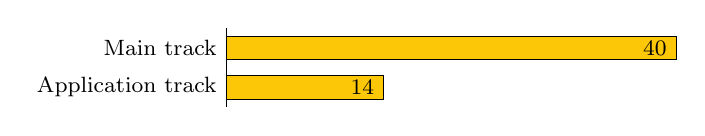
\begin{tikzpicture}
      \draw (0,-.25) -- (0,.75);
      \node [left] at (0,.5) {\footnotesize Main track};
      \node [left] at (0,0) {\footnotesize Application track};
      \draw [fill=yellow!80!red] (0,.35) rectangle (5.714285714,.65);
      \node [left] at (5.714285714,.5) {\footnotesize 40};
      \draw [fill=yellow!80!red] (0,-.15) rectangle (2,.15);
      \node [left] at (2,0) {\footnotesize 14};
    \end{tikzpicture}
  \item Benchmarks:\\
    \smallskip
    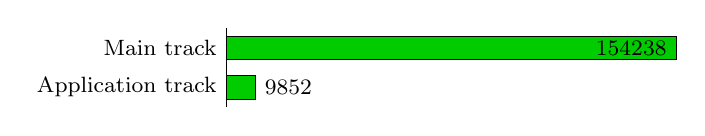
\begin{tikzpicture}
      \draw (0,-.25) -- (0,.75);
      \node [left] at (0,.5) {\footnotesize Main track};
      \node [left] at (0,0) {\footnotesize Application track};
      \draw [fill=green!80!black] (0,.35) rectangle (5.714285714,.65);
      \node [left] at (5.714285714,.5) {\footnotesize 154238};
      \draw [fill=green!80!black] (0,-.15) rectangle (0.365001769,.15);
      \node [right] at (0.365001769,0) {\footnotesize 9852};
    \end{tikzpicture}
  \end{itemize}

  \medskip

  \structure{Record numbers} of solvers, logics, and benchmarks!
\end{frame}

%%%%%%%%%%%%%%%%%%%%%%%%%%%%%%%%%%%%%%%%%%%%%%%%%%%%%%%%%%%%%%%%%%%%%%%%%%%%%%%%

\begin{frame}{Job Pairs}
  \begin{itemize}
  \item \structure{1,028,615} job pairs executed (+ some repeats)
  \item $\sim$ \structure{5 days $\times$ 150 nodes $\times$ 2
    processors/node} of compute time
  \end{itemize}

  \bigskip

  \begin{center}
    \usebeamercolor{structure}
    \begin{tikzpicture}
      \draw [gray] (0,0) -- (7,0);
      \draw [gray] (0,.9) -- (7,.9);
      \draw [gray] (0,1.8) -- (7,1.8);
      \draw [gray] (0,2.7) -- (7,2.7);
      \node [left,gray] at (0,0) {\tiny 0};
      \node [left,gray] at (0,.9) {\tiny 300,000};
      \node [left,gray] at (0,1.8) {\tiny 600,000};
      \node [left,gray] at (0,2.7) {\tiny 900,000};
      \draw [fill=fg!30!white] (1,0) rectangle (3,1.019142);
      \draw [fill=fg] (4,0) rectangle (6,3.085845);
      \node [below,gray] at (2,0) {\footnotesize SMT-COMP 2014};
      \node [below] at (5,0) {\footnotesize SMT-COMP 2015};
    \end{tikzpicture}\qquad${}$
  \end{center}
  More than \structure{3 times} as many job pairs as in 2014!
\end{frame}

%%%%%%%%%%%%%%%%%%%%%%%%%%%%%%%%%%%%%%%%%%%%%%%%%%%%%%%%%%%%%%%%%%%%%%%%%%%%%%%%

\begin{frame}{StarExec}
  \begin{itemize}
  \item All job pairs executed on StarExec
  \item Over 9,000 job pairs/hour completed
  \end{itemize}

  \medskip

  \begin{center}
    {\Large\structure{StarExec worked great}}
  \end{center}

  \medskip

  \begin{itemize}
  \item Thanks to Aaron Stump for prompt help when problems or
    questions arose
  \item $\sim$ 20 feature requests and (minor) bug reports submitted
    to the StarExec developers
  \end{itemize}
\end{frame}

%%%%%%%%%%%%%%%%%%%%%%%%%%%%%%%%%%%%%%%%%%%%%%%%%%%%%%%%%%%%%%%%%%%%%%%%%%%%%%%%

\begin{frame}{Machine Specifications}
  Hardware:
  \begin{itemize}
  \item Intel Xeon CPU E5-2609 @ 2.4 GHz, 10 MB cache
  \item 2 processors per node, 4 cores per processor
  \item Main memory capped at 60~GB per job pair
  \end{itemize}

  \medskip

  Software:
  \begin{itemize}
  \item Red Hat Enterprise Linux Workstation release 6.3
  \item Kernel 2.6.32-431, gcc 4.4.6, glibc 2.12 ($\sim$ 2009-2011)
  \item Virtual machine image available before the competition
  \end{itemize}

  \bigskip

  Problems with \structure{missing libraries} (due to dynamic linking)
  in several solvers resolved during pre-competition testing in early
  June.
\end{frame}

%%%%%%%%%%%%%%%%%%%%%%%%%%%%%%%%%%%%%%%%%%%%%%%%%%%%%%%%%%%%%%%%%%%%%%%%%%%%%%%%

\begin{frame}{Benchmarks and Logics}
  \begin{itemize}
  \item Almost 60,000 new benchmarks added to SMT-LIB, thanks to
    \todo{\$BENCHMARK\_CONTRIBUTORS}:\\
    \smallskip
    \begin{center}
      \usebeamercolor{structure}
      \begin{tikzpicture}[yscale=1.2]
        \draw [gray] (0,0) -- (7,0);
        \draw [gray] (0,.5) -- (7,.5);
        \draw [gray] (0,1) -- (7,1);
        \draw [gray] (0,1.5) -- (7,1.5);
        \draw [gray] (0,2) -- (7,2);
        \node [left,gray] at (0,0) {\tiny 0};
        \node [left,gray] at (0,1) {\tiny 100,000};
        \node [left,gray] at (0,2) {\tiny 200,000};
        \draw [fill=cyan!20!white] (1,0) rectangle (3,0.09925);
        \draw [fill=fg!30!white] (1,0.0925) rectangle (3,1.47573);
        \draw [fill=cyan] (4,0) rectangle (6,0.10019);
        \draw [fill=fg] (4,0.10019) rectangle (6,2.06394);
        \node [above,white] at (5,0.10019) {\tiny incremental};
        \node [above] at (5,2.06394) {\tiny non-incremental};
        \node [below,gray] at (2,0) {\small 2014};
        \node [below] at (5,0) {\small 2015};
      \end{tikzpicture}\qquad${}$
    \end{center}
  \item Six new logics, including two new \structure{floating-point}
    logics
  \item Thanks to Clark Barrett for curation and uploading
  \end{itemize}
\end{frame}

%%%%%%%%%%%%%%%%%%%%%%%%%%%%%%%%%%%%%%%%%%%%%%%%%%%%%%%%%%%%%%%%%%%%%%%%%%%%%%%%

\begin{frame}{Benchmark Curation}
  \begin{itemize}
  \item Sanity checks
    \begin{itemize}
    \item One satisfiability check per benchmark in main track
    \item Status information set before satisfiability check
    \end{itemize}
  \item Verify benchmark signature against logic set
  \item Remove unused symbols
  \item Improve logic settings
  \end{itemize}
\end{frame}

%%%%%%%%%%%%%%%%%%%%%%%%%%%%%%%%%%%%%%%%%%%%%%%%%%%%%%%%%%%%%%%%%%%%%%%%%%%%%%%%

\begin{frame}{Eligible Benchmarks}
  \begin{center}
    \usebeamercolor{structure}
    \begin{tikzpicture}[yscale=2]
      \draw [gray] (0,0) -- (3.75,0); \draw [gray] (4.25,0) -- (8,0);
      \draw [gray] (0,.5) -- (3.75,.5); \draw [gray] (4.25,.5) -- (8,.5);
      \draw [gray] (0,1) -- (3.75,1); \draw [gray] (4.25,1) -- (8,1);
      \draw [gray] (0,1.5) -- (3.75,1.5);
      \draw [gray] (0,2) -- (3.75,2);
      \node [left,gray] at (0,0) {\tiny 0};
      \node [left,gray] at (0,1) {\tiny 100,000};
      \node [left,gray] at (0,2) {\tiny 200,000};
      \node [right,gray] at (8,0) {\tiny 0};
      \node [right,gray] at (8,.5) {\tiny 5,000};
      \node [right,gray] at (8,1) {\tiny 10,000};
      \draw [fill=lightgray] (1,1.66204) rectangle (3,1.96375);
      \draw [fill=orange] (1,1.54238) rectangle (3,1.66204);
      \draw [fill=fg] (1,0) rectangle (3,1.54238);
      \draw [fill=lightgray] (5,0.9852) rectangle (7,1.0019);
      \draw [fill=fg] (5,0) rectangle (7,0.9852);
      \node at (2,1.812895) {\tiny status unknown};
      \node at (2,1.60221) {\tiny partial operations};
      \node [white] at (2,0.77119) {\tiny eligible};
      \node [above] at (6,0.99355) {\tiny status unknown};
      \node [white] at (6,0.4926) {\tiny eligible};
      \node [below] at (2,0) {\small Main track};
      \node [below] at (6,0) {\small Application track};
    \end{tikzpicture}
  \end{center}

  All eligible benchmarks were used for the competition.  There was
  \structure{no further selection}.
\end{frame}

%%%%%%%%%%%%%%%%%%%%%%%%%%%%%%%%%%%%%%%%%%%%%%%%%%%%%%%%%%%%%%%%%%%%%%%%%%%%%%%%

% Source: http://www.clker.com/clipart-quality-control-approved-1.html
\logo{
\includegraphics[width=2.5cm]{quality-control-approved}}

\begin{frame}{Competition Tools Improved}
  \begin{itemize}
  \item Fixed an issue where the \structure{trace executor} would
    sometimes not count correct solver responses on partially solved
    incremental benchmarks. (Thanks to Kshitij Bansal for reporting
    this.)

    \bigskip

  \item Fixed several issues in the \structure{benchmark scrambler}
    that caused invalid output in the presence of variable shadowing.
  \end{itemize}

  \bigskip
\end{frame}

\logo{}

%%%%%%%%%%%%%%%%%%%%%%%%%%%%%%%%%%%%%%%%%%%%%%%%%%%%%%%%%%%%%%%%%%%%%%%%%%%%%%%%

\begin{frame}{Scrambling}

\end{frame}

%%%%%%%%%%%%%%%%%%%%%%%%%%%%%%%%%%%%%%%%%%%%%%%%%%%%%%%%%%%%%%%%%%%%%%%%%%%%%%%%

%%%%%%%%%%%%%%%%%%%%%%%%%%%%%%%%%%%%%%%%%%%%%%%%%%%%%%%%%%%%%%%%%%%%%%%%%%%%%%%%

\begin{frame}{Evolution of Benchmarks: Breakdown}

\end{frame}

%%%%%%%%%%%%%%%%%%%%%%%%%%%%%%%%%%%%%%%%%%%%%%%%%%%%%%%%%%%%%%%%%%%%%%%%%%%%%%%%

\begin{frame}{Evolution of Tool Participation: Breakdown}

\end{frame}

%%%%%%%%%%%%%%%%%%%%%%%%%%%%%%%%%%%%%%%%%%%%%%%%%%%%%%%%%%%%%%%%%%%%%%%%%%%%%%%%

\begin{frame}{Further Thoughts}
  Benchmarks:
  \begin{itemize}
  \item Still more benchmarks needed, especially for small divisions
  \item Resolve semantics of partial operations, e.g., {\tt bvdiv},
    {\tt fp.min}
  \end{itemize}

  \medskip

  Solvers:
  \begin{itemize}
  \item Parallelism
  \end{itemize}

  \medskip

  Competition:
  \begin{itemize}
  \item Relative weight of benchmarks and benchmark families
  \item Separate measure of performance on quick jobs
  \item Additional tracks, e.g., unsat-core, proofs
  \end{itemize}

  \medskip

  Teams:
  \begin{itemize}
  \item \structure{Congratulations on your accomplishments!}
  \item \structure{Thanks for your participation!}
  \end{itemize}
\end{frame}

%%%%%%%%%%%%%%%%%%%%%%%%%%%%%%%%%%%%%%%%%%%%%%%%%%%%%%%%%%%%%%%%%%%%%%%%%%%%%%%%

\end{document}

%%%%%%%%%%%%%%%%%%%%%%%%%%%%%%%%%%%%%%%%%%%%%%%%%%%%%%%%%%%%%%%%%%%%%%%%%%%%%%%%

% Local Variables:
% ispell-local-dictionary: "american"
% mode: LaTeX
% mode: flyspell
% LocalWords: curation logics satisfiability Tjark
% End:
